% Algorithm 1 routing decision schematic.
%
% Provenance: bound by ci/illustration_lineage.json to the Algorithm 1
% block at main.tex:96-114. The block is pseudocode; this schematic
% exposes the decision-tree shape: parse -> compute (rho-hat, delta in
% parallel) -> screened cost -> three-way route.
%
% Composition draft via gpt-5.4-image-2 (see
% supplementary/illustrations/algorithm1_routing_draft.png and the
% spec at algorithm1_routing_spec.md). Final asset is this hand-
% authored TikZ; the certificate trusts only the deterministic redraw.
%
% Claim scope: schematic illustration only; not empirical evidence.
%
% Layout note: every node uses an explicit (x, y) position rather than
% `below=of` chained placement. Earlier versions used relative offsets
% which caused the screened-cost box to collide vertically with the
% rho/budget parallel pair once box widths were grown to accommodate
% the longer formulas. Explicit coordinates make the layout deterministic.

\begin{figure}[!htb]
\centering
\resizebox{\linewidth}{!}{%
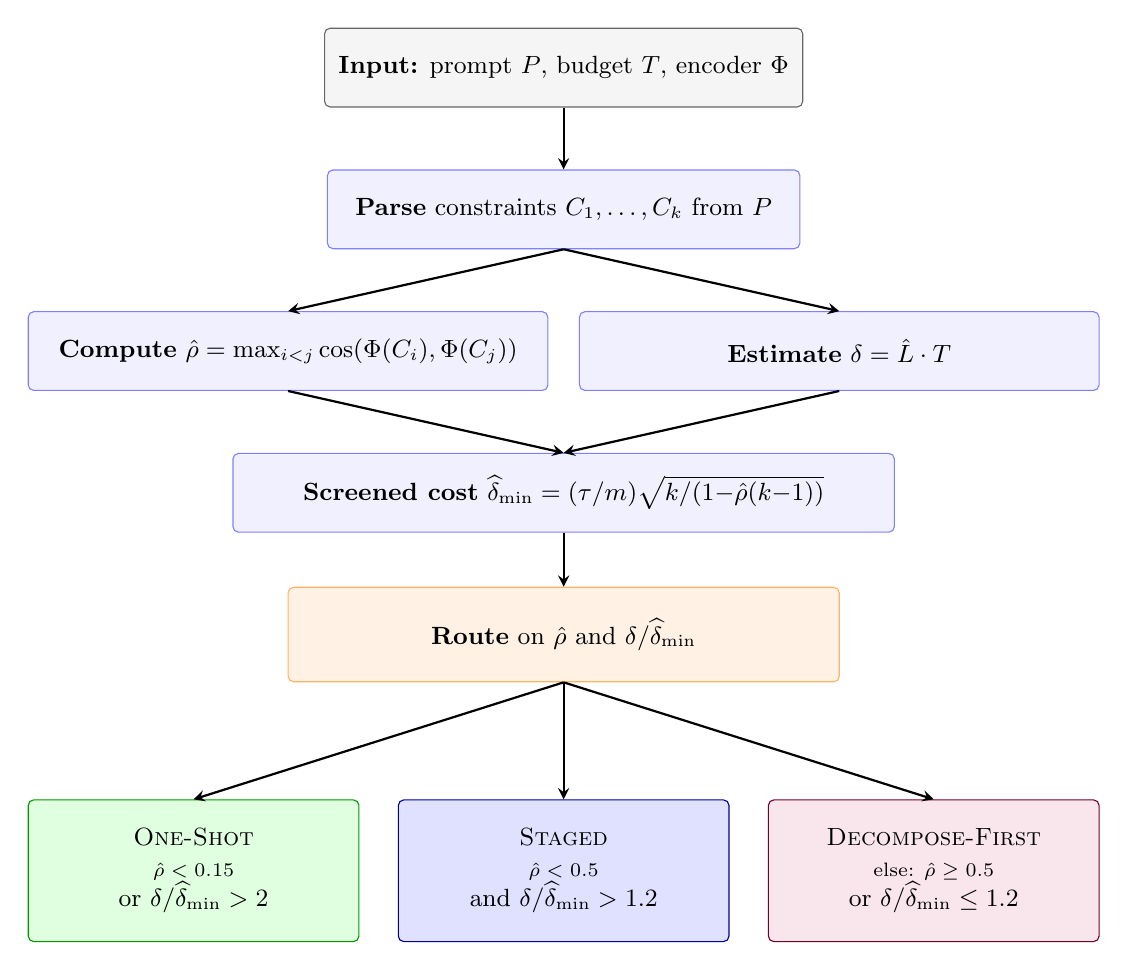
\begin{tikzpicture}[
    font=\small,
    box/.style={draw, rounded corners=2pt, minimum height=10mm, align=center, inner sep=5pt, fill=white, draw=black!60},
    inputbox/.style={box, fill=gray!8, minimum width=60mm},
    parsebox/.style={box, fill=blue!6, draw=blue!50, minimum width=60mm},
    parallel/.style={box, fill=blue!6, draw=blue!50, minimum width=66mm},
    costbox/.style={box, fill=blue!6, draw=blue!50, minimum width=84mm},
    decisionbox/.style={box, fill=orange!10, draw=orange!60, minimum width=70mm, minimum height=12mm},
    routebox/.style={box, minimum width=42mm, minimum height=18mm, align=center},
    oneshot/.style={routebox, fill=green!12, draw=green!60!black},
    staged/.style={routebox, fill=blue!12, draw=blue!60!black},
    decomp/.style={routebox, fill=purple!10, draw=purple!60!black},
    arr/.style={->, thick, >=stealth},
    cond/.style={font=\scriptsize, color=black!70, align=center},
]
    % Row 1: input
    \node[inputbox] (inp) at (0, 0) {\textbf{Input:} prompt $P$, budget $T$, encoder $\Phi$};

    % Row 2: parse
    \node[parsebox] (parse) at (0, -1.8) {\textbf{Parse} constraints $C_1, \ldots, C_k$ from $P$};

    % Row 3: parallel pair (rho on left, budget on right)
    \node[parallel] (rho)    at (-3.5, -3.6) {\textbf{Compute} $\hat{\rho} = \max_{i<j}\cos(\Phi(C_i),\Phi(C_j))$};
    \node[parallel] (budget) at ( 3.5, -3.6) {\textbf{Estimate} $\delta = \hat{L} \cdot T$};

    % Row 4: screened cost (below the parallel pair, centered)
    \node[costbox] (cost) at (0, -5.4) {\textbf{Screened cost} $\widehat{\delta}_{\min} = (\tau/m)\sqrt{k/(1{-}\hat{\rho}(k{-}1))}$};

    % Row 5: route decision
    \node[decisionbox] (route) at (0, -7.2) {\textbf{Route} on $\hat{\rho}$ and $\delta/\widehat{\delta}_{\min}$};

    % Row 6: three terminals.  Each terminal carries its routing condition
    % inside the box (top line = action name, bottom lines = condition) so
    % the condition text cannot overflow the box bounds.
    \node[oneshot] (oneshot) at (-4.7, -10.2) {\textsc{One-Shot} \\ \scriptsize $\hat{\rho}<0.15$ \\ or $\delta/\widehat{\delta}_{\min}>2$};
    \node[staged]  (staged)  at ( 0.0, -10.2) {\textsc{Staged} \\ \scriptsize $\hat{\rho}<0.5$ \\ and $\delta/\widehat{\delta}_{\min}>1.2$};
    \node[decomp]  (decomp)  at ( 4.7, -10.2) {\textsc{Decompose-First} \\ \scriptsize else: $\hat{\rho}\ge 0.5$ \\ or $\delta/\widehat{\delta}_{\min}\le 1.2$};

    % Arrows
    \draw[arr] (inp.south) -- (parse.north);
    \draw[arr] (parse.south) -- (rho.north);
    \draw[arr] (parse.south) -- (budget.north);
    \draw[arr] (rho.south) -- (cost.north);
    \draw[arr] (budget.south) -- (cost.north);
    \draw[arr] (cost.south) -- (route.north);
    \draw[arr] (route.south) -- (oneshot.north);
    \draw[arr] (route.south) -- (staged.north);
    \draw[arr] (route.south) -- (decomp.north);
\end{tikzpicture}
}
\caption{Algorithm~\ref{alg:routing} as a decision tree (schematic). The screening statistic $\hat{\rho}$ and budget ratio $\delta/\widehat{\delta}_{\min}$ are computed from the prompt before generation, then composed at a single routing junction with three terminal regimes. The conditions printed above each terminal are exactly those in lines 6--12 of Algorithm~\ref{alg:routing}. Provenance: \texttt{ci/illustration\_lineage.json}; draft via gpt-5.4-image-2; final asset is hand-authored TikZ. Schematic illustration only; not empirical evidence.}
\label{fig:algorithm1_routing}
\end{figure}
